\documentclass[12pt]{beamer}
\usetheme{Warsaw}
\usepackage[utf8]{inputenc}
\usepackage{amsmath}
\usepackage{amsfonts}
\usepackage{amssymb}
\author{Piyush and Neil}
\title{Linear Algebra}
\subtitle{Q.36}
\institute{IIT Hyderabad}
%\title{}
%\setbeamercovered{transparent} 
%\setbeamertemplate{navigation symbols}{} 
%\logo{} 
%\institute{} 
%\date{} 
%\subject{} 
\begin{document}

\begin{frame}
\titlepage
\end{frame}

%\begin{frame}
%\tableofcontents
%\end{frame}

\begin{frame}{Question 31}
Find the equation of the tangent to the circle at the point [$\begin{array}{c}
1 \\ 
-1
\end{array}$] whose centre is point of intersection of straight lines [$\begin{array}{cc}
2 & 1
\end{array}]x = 3$ and [$\begin{array}{cc}
1 & -1
\end{array}]x = 1$


\end{frame}

\begin{frame}{Solution}
\begin{itemize}
  \item Let A=[$\begin{array}{c}
2 \\ 
1
\end{array}$] and B=$[\begin{array}{c}
1 \\ 
-1
\end{array}]$
  \item Let O be the solution of Ax=3 and Bx=1
  This can be written as $[\begin{array}{cc}
  2 & 1 \\ 
  1 & -1
  \end{array}$]x = $[\begin{array}{c}
3 \\ 
1
\end{array}]$
\item Therefore, O = $[\begin{array}{cc}
  2 & 1 \\ 
  1 & -1
  \end{array}]^{-1}[\begin{array}{c}
3 \\ 
1
\end{array}]$
\item O = $[\begin{array}{c}
\frac{4}{3} \\ 
\frac{1}{3}
\end{array}]$
\end{itemize}


\end{frame}

\begin{frame}{Solution}
\begin{itemize}
\item Given a point P on circle as P=$[\begin{array}{c}
1 \\ 
-1
\end{array}]$ and we have O=$[\begin{array}{c}
\frac{4}{3} \\ 
\frac{1}{3}
\end{array}]$
\item Let us define matrix T=$[\begin{array}{cc}
O & P
\end{array}] = [\begin{matrix}
\frac{4}{3} & 1 \\ 
\frac{1}{3} & -1
\end{matrix}]$
\item The direction vector OP is given by D = P-O = [T]$[\begin{array}{c}
-1 \\ 
1
\end{array}] = [\begin{matrix}
\frac{4}{3} & 1 \\ 
\frac{1}{3} & -1
\end{matrix}][\begin{array}{c}
-1 \\ 
1
\end{array}]$ = $[\begin{array}{c}
-\frac{1}{3} \\ 
-\frac{4}{3}
\end{array}]$ which is a radial vector.

 
\end{itemize}

\end{frame}

\begin{frame}{Solution}
\begin{itemize}
\item The direction vector for tangent line will be the normal vector to radial vector. Let normal vector = N
\item By definition, $N^{T}D = 0$
\item Therefore, N = $[\begin{matrix}
0 & 1 \\ 
-1 & 0
\end{matrix}]$[D] = $[\begin{matrix}
0 & 1 \\ 
-1 & 0
\end{matrix}][\begin{array}{c}
-\frac{1}{3} \\ 
-\frac{4}{3}
\end{array}]$ = $[\begin{array}{c}
-\frac{4}{3} \\ 
\frac{1}{3}
\end{array}]$
 \item Tangent line : x = P + (t)N
 
 \vspace{0.5em} 
 \item x = $[\begin{array}{c}
1 \\ 
-1
\end{array}] + (t)[\begin{array}{c}
-\frac{4}{3} \\ 
\frac{1}{3}
\end{array}]$

\end{itemize}

\end{frame}

\begin{frame}{Figure}
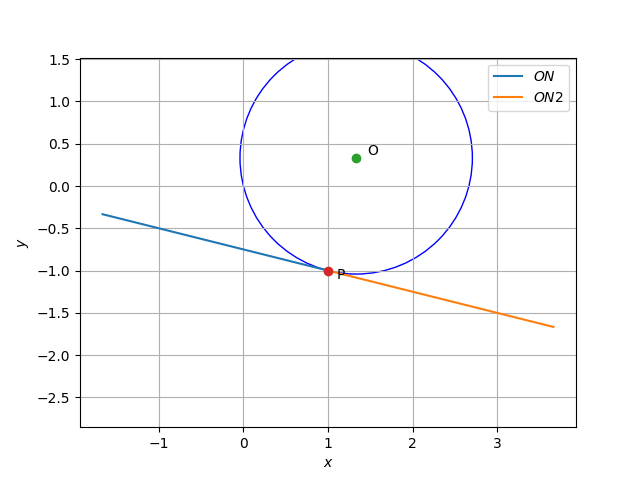
\includegraphics[scale=0.7]{Figure_1.png}

\end{frame}





\end{document}